\chapter{Predicting Football Matches}
\label{ch:playerkern}

In this chapter\footnote{%
This chapter is based on \citet*{maystre2016player}.},
we shift our attention from human choices to sports outcomes.
In particular, we draw attention to a connection between skill-based models of game outcomes (built on the Bradley--Terry model) and Gaussian-process classification models.
The Gaussian-process perspective enables
\begin{enuminline}
\item a principled way of dealing with uncertainty and
\item rich models, specified through kernel functions.
\end{enuminline}
Using this connection, we tackle the problem of predicting outcomes of football matches between national teams.
We develop a \emph{player kernel} that relates any two football matches through the players lined up on the field.
This makes it possible to share knowledge gained from observing matches between clubs (available in large quantities) and matches between national teams (available only in limited quantities).
We evaluate our approach on the Euro 2008, 2012 and 2016 final tournaments.


%%%%%%%%%%%%%%%%%%%%%%%%%%%%%%%%
\section{Introduction}
\label{fi:sec:intro}

Markov chains have been used in recent work to aggregate inconsistent outcomes of pairwise comparisons and (partial) rankings \citep{dwork2001rank, negahban2012iterative, azari2013generalized}.
The idea is to build a Markov chain that is biased towards items that have won often, and to reduce the problem of ranking items to that of finding the \emph{stationary distribution} of the chain (the ranking is then induced by the items' stationary probabilities).
In this chapter, we highlight a connection between the MLE of models based on Luce's choice axiom and the stationary distribution of a Markov chain parametrized by the observed choices.
By formalizing this link, we unify previous algorithms and explicate them from an ML inference perspective.
Beyond this, the link suggests two new algorithms for parameter inference.
First, we develop a simple, consistent and computationally efficient spectral algorithm that is applicable to a wide range of models derived from Luce's choice axiom.
The exact formulation of the Markov chain used in the algorithm is distinct from related work \citep{negahban2012iterative, azari2013generalized} and achieves a significantly better statistical efficiency at no additional computational cost.
Second, we observe that with a small adjustment, the algorithm can be used iteratively, and it then converges to the MLE.
An evaluation on five real-world datasets reveals that it runs consistently faster than competing approaches and has a more predictable performance that does not depend on the structure of the data.
The key step, finding a stationary distribution, can be offloaded to commonly available linear-algebra primitives, which makes our algorithms  scale well.
The method we propose is intuitively pleasing, simple to understand and implement, and it outperforms the state of the art, hence we believe that it is highly useful to practitioners.

\paragraph{Outline of the Chapter}
We begin by introducing some notations and presenting a few useful facts about the MLE and about Markov chains.
In Section~\ref{fi:sec:relwork}, we discuss related work.
In Section~\ref{fi:sec:algorithms}, we present our algorithms, and in Section~\ref{fi:sec:experiments} we evaluate them on synthetic and real-world data.


\subsection{Maximum-Likelihood Estimate}
\label{fi:sec:mle}

%The log-likelihood \eqref{fi:eq:loglik} is not concave in $\bm{\gamma}$ (it can be made strictly concave using a simple reparametrization), but we briefly show in the supplementary material that it admits a unique stationary point, at the ML estimate $\bm{\gamma}^\star$.

Suppose that we collect $M$ independent choice observations in the multiset $\mathcal{D} = \{(c_m, \mathcal{A}_m) : m = 1, \ldots, M\}$.
Each observation consists of a choice $c_m$ among a set of alternatives $\mathcal{A}_m$;
we say that \emph{$i$ wins over $j$} and denote by $i \succ j$ whenever $i, j \in \mathcal{A}_m$ and $c_m = i$.
We postulate that the choices are generated from Luce's choice model, and for simplicity we denote the model parameter associated with item $c_m$ by $\gamma_m$.
From~\eqref{in:eq:luce}, it follows that the log-likelihood of parameters $\bm{\gamma}$ given observations $\mathcal{D}$ is given by
\begin{align}
\label{fi:eq:loglik}
\ell(\bm{\gamma}) = \sum_{m = 1}^M \bigg[ \log \gamma_m - \log{\sum_{j \in \mathcal{A}_m} \gamma_j} \bigg].
\end{align}
In order to ensure that the parameters are likelihood-identifiable, we assume without loss of generality that $\sum_i \gamma_i = 1$.
Next, we introduce a new object.

\begin{definition}[comparison graph]
The \emph{comparison graph} $\mathcal{G}_{\mathcal{D}} = (\mathcal{V}, \mathcal{E})$ is a directed graph with $\mathcal{V} = [N]$ and $(j, i) \in \mathcal{E}$ if and only if $i$ wins at least once over $j$ in $\mathcal{D}$.
\end{definition}

The existence and uniqueness of the MLE is completely determined by the connectivity of $\mathcal{G}_{\mathcal{D}}$, as the following well-known theorem shows.

\begin{theorem}[\citealp{zermelo1928berechnung, ford1957solution, hunter2004mm}]
\label{fi:thm:mlboth}
The likelihood function~\eqref{fi:eq:loglik} admits a unique maximizer $\bm{\gamma}^\star \in \mathbf{R}^N_{>0}$ such that $\sum_i \gamma^\star_i = 1$ if and only if $\mathcal{G}_{\mathcal{D}}$ is strongly connected.
\end{theorem}

Throughout this chapter, we will assume that $\mathcal{G}_{\mathcal{D}}$ is strongly connected.
In practice, if this assumption does not hold, we can consider each strongly-connected component separately.
Finally, note that even though $\ell(\bm{\gamma})$ admits a unique maximizer, it is not concave.
However, reparametrizing the model using $\theta_i \doteq \log \gamma_i$, the log-likelihood becomes
\begin{align*}
\ell(\bm{\theta}) = \sum_{m = 1}^M \bigg[ \theta_m - \log{\sum_{j \in \mathcal{A}_m} \exp \theta_j} \bigg],
\end{align*}
which is strictly concave in $\bm{\theta}$ (when $\mathcal{G}_{\mathcal{D}}$ is strongly connected).
Furthermore, for all $i \in [N]$,
\begin{align*}
\frac{\partial \ell}{\partial \gamma_i}
  = \frac{\partial \ell}{\partial \theta_i} \cdot \frac{\partial \theta_i}{\partial \gamma_i}
  = \frac{\partial \ell}{\partial \theta_i} \cdot \frac{1}{\gamma_i}
\quad \implies \quad
\frac{\partial \ell}{\partial \theta_i} = 0 \iff \frac{\partial \ell}{\partial \gamma_i} = 0.
\end{align*}
As the strictly concave function $\ell({\bm{\theta}})$ has a single stationary point, it follows that $\ell(\bm{\gamma})$ has a single stationary point at $\bm{\gamma}^\star$.


\subsection{Markov Chains}

We represent a finite, continuous-time Markov chain on $N$ states by a directed graph $\mathcal{G} = (\mathcal{V}, \mathcal{E})$, where $\mathcal{V} = [N]$ and $\mathcal{E}$ is the set of transitions with positive rate\footnote{%
Our exposition of Markov chains is succinct, and the interested reader is encouraged to consult \citet{levin2008markov} for a more thorough exposition.}.
If $\mathcal{G}$ is strongly connected, the Markov chain is said to be ergodic and admits a unique \emph{stationary distribution} $\bm{\pi} \in \mathbf{R}^N_{>0}$, $\sum_i \pi_i = 1$.
The \emph{global balance equations} relate the transition rates $\{ \lambda_{ij} \}$ to the stationary distribution as follows:
\begin{align}
\label{fi:eq:balance}
\sum_{j \ne i} \pi_i \lambda_{ij} = \sum_{j \ne i} \pi_j \lambda_{ji} \quad \forall i.
\end{align}
The stationary distribution is therefore invariant to changes in the time scale, i.e., to a rescaling of the transition rates.
Given transition rates $\bm{\Lambda} = [\lambda_{ij}]$, finding the stationary distribution $\bm{\pi}$ can be implemented in several different ways.
We distinguish implementations based on whether they consider a continuous-time or a discrete-time perspective on Markov chains.

\paragraph{Continuous-Time Perspective}
Let $\bm{Q}$ be the infinitesimal generator matrix of the Markov chain, i.e., $q_{ij} \doteq \lambda_{ij}$ and $q_{ii} \doteq - \sum_{j} \lambda_{ij}$.
The stationary distribution satisfies $\bm{\pi}^\Tr \bm{Q} = 0$; this is simply a matrix formulation of the global balance equations~\eqref{fi:eq:balance}.
Therefore, one approach to finding the steady-state distribution is to compute the rank-$1$ left nullspace of $\bm{Q}$.
This can be done, e.g., by LU decomposition, a basic linear-algebra primitive.
In the case where $\bm{Q}$ is dense, the running time of a typical implementation is $\BigO{N^3}$, but highly optimized parallel implementations such as that provided by LAPACK \citep{anderson1999lapack} are commonly available.
In the sparse case, LU decomposition can be done significantly faster using adapted algorithms, such as that of \citet{demmel1999supernodal}.

\paragraph{Discrete-Time Perspective}
Let $\epsilon < 1 / \max_i |q_{ii}|$, then $\bm{P} = \bm{I} + \epsilon \bm{Q}$ is the transition matrix of a discrete-time Markov chain that satisfies $\bm{\pi}^\Tr \bm{P} = \bm{\pi}$.
In this case, finding the steady-state distribution is equivalent to finding the left eigenvector associated to the leading eigenvalue of the transition matrix $\bm{P}$.
This is also a well-studied linear algebra problem for which plenty of efficient, off-the-shelf algorithms exist.
For example, power iteration methods can find the eigenvector in a few (sparse) matrix multiplications.
Beyond these well-known algorithms, recently-proposed randomized approaches such as that of \citet{halko2011finding} make it possible to scale to very large problem sizes ($N \sim 10^6$ or more).

Both the continuous-time and the discrete-time perspectives yield exactly the same resulting stationary distribution, and the algorithms presented in this paper are oblivious to this choice.

%%%%%%%%%%%%%%%%%%%%%%%%%%%%%%%%%%%%%%%%%%%%%%%%%%%%%%%%%%%%%%%%%%%%%%%%%
\section{Related Work}  %%%%%%%%%%%%%%%%%%%%%%%%%%%%%%%%%%%%%%%%%%%%%%%%%
\label{cr:sec:relwork}

A variant of the network choice model was recently introduced by \citet{kumar2015inverting}, in an article that lays much of the groundwork for this chapter.
Their generative model of traffic and the parametrization of transition probabilities based on Luce's axiom form the basis of our work.
\citeauthor{kumar2015inverting} define the \emph{steady-state inversion} problem as follows:
Given a graph $\mathcal{G}$ and a target stationary distribution, find transition probabilities that lead to the desired stationary distribution.
This problem formulation assumes that $\mathcal{G}$ satisfies restrictive structural properties (strong-connectedness, aperiodicity) and is valid only asymptotically, when the sequences of choices made by users are very long.
Our formulation is, in contrast, more general.
In particular, we eliminate any assumptions about the structure of $\mathcal{G}$ and cope with finite data in a principled way---in fact, our derivations are valid for choice sequences of any length.
One of our contributions is to explain the steady-state inversion problem in terms of (asymptotic) maximum-likelihood inference in the network choice model.
Furthermore, the statistical viewpoint that we develop also leads to
\begin{enuminline}
\item a robust regularization scheme, and
\item a simple and efficient EM-type inference algorithm.
\end{enuminline}
These important extensions make the model easier to apply to real-world data.

\paragraph{Luce's Choice Axiom}
The general problem of estimating parameters of models based on Luce's axiom has received considerable attention.
Several decades before Luce's seminal book \citep{luce1959individual}, \citet{zermelo1928berechnung} proposed a model and an algorithm that estimates the strengths of chess players based on pairwise comparison outcomes (his model would later be rediscovered by \citet{bradley1952rank}).
More recently, \citet{hunter2004mm} explained \citeauthor{zermelo1928berechnung}'s algorithm from the perspective of the minorization-maximization (MM) method.
This method is easily generalized to other models that are based on Luce's axiom, and it yields simple, provably convergent algorithms for maximum-likelihood (ML) or maximum-a-posteriori point estimates.
\citet{caron2012efficient} observe that these MM algorithms can be further recast as expectation-maximization (EM) algorithms by introducing suitable latent variables.
They use this observation to derive Gibbs samplers for a wide family of models.
We take advantage of this long line of work in Section~\ref{cr:sec:inference} when developing an inference algorithm for the network choice model.
In recent years, several authors have also analyzed the sample complexity of the ML estimate in Luce's choice model \citep{hajek2014minimax, vojnovic2016parameter} and investigated alternative spectral inference methods \citep{negahban2012iterative, azari2013generalized, maystre2015fast}.
Some of these results could be applied to our setting, but in general they require observing choices among well-identified sets of alternatives.
Finally, we note that models based on Luce's axiom have been successfully applied to problems ranging from ranking players based on game outcomes \citep{zermelo1928berechnung, elo1978rating} to understanding consumer behavior based on discrete choices \citep{mcfadden1973conditional}, and to discriminating among multiple classes based on the output of pairwise classifiers \citep{hastie1998classification}.

\paragraph{Network Analysis}
Understanding the preferences of users in networks is of significant interest in many domains.
For brevity, we focus on literature related to hyperlink graphs.
A method that has undoubtedly had a tremendous impact in this context is PageRank \citep{brin1998anatomy}.
PageRank computes a set of scores that are proportional to the amount of time a surfer, who clicks on links randomly and uniformly, spends at each node.
These scores are based only on the structure of the graph.
The network choice model presented in this chapter appears similar at first, but tackles a different problem.
In addition to the structure of the graph, it uses the traffic at each page, and computes a set of scores that reflect the (non-uniform) probability of clicking on each link.
Nevertheless, there are striking similarities in the implementation of the respective inference algorithms (see Section~\ref{cr:sec:experiments}).
The HOTness method proposed by \citet{tomlin2003new} is somewhat related, but tries to tackle a harder problem.
It attempts to estimate jointly the traffic and the probability of clicking on each link, by using a maximum-entropy approach.
At the other end of the spectrum, BrowseRank \citep{liu2008browserank} uses detailed data collected in users' browsers to improve on PageRank.
Our method uses only marginal traffic data that can be obtained without tracking users.
%In the context of mobility analysis, we mention that \citet{ashbrook2003using} and \citet{kafsi2015traveling}

\section{Methods}
\label{pk:sec:methods}

In this section, we first show how the model of pairwise comparisons proposed by \citet{zermelo1928berechnung} and popularized by \citet{bradley1952rank} and \citet{elo1978rating} can be expressed in the Gaussian process framework.
Second, we present the player kernel, a covariance function that relates matches through lineups.


\subsection{Pairwise Comparisons as Gaussian Process Classification}

Suppose that we observe outcomes of comparisons between two objects (e.g., two players or two teams) in a universe of objects denoted $1, \ldots, M$.
We begin by restricting ourselves to binary outcomes, i.e., we assume that one of the two objects wins.
\citet{zermelo1928berechnung} postulates that each object $u$ can be represented by a parameter $w_u \in \mathbf{R}_{>0}$, indicative of its relative chances of winning against an opponent.
Given these parameters, the probability of observing the outcome ``$u$ wins against $v$'' (denoted by $u \succ v$) is given by $w_u / (w_u + w_v)$.
Using the reparametrization $w_u = e^{s_u}$, this can be rewritten as
\begin{align}
\label{pk:eq:logistic}
P(u \succ v) = \frac{1}{1 + \exp[-(s_u - s_v)]} = \frac{1}{1 + \exp(- \bm{s}^\top \bm{x})},
\end{align}
where $\bm{s} = [s_i]$ and $\bm{x} \in \mathbf{R}^M$ is such that $x_u = 1$, $x_v = -1$ and $x_i = 0$ for $i \ne u, v$.
As such, the pairwise comparison model can be seen as a special case of logistic regression, where the feature vector simply indicates the winning and losing objects.
Furthermore, logistic regression is itself a special case of Gaussian process classification \cite[Ch. 3]{rasmussen2006gaussian}.
A Gaussian process $f(\bm{x}) \sim \mathcal{GP}(m(\bm{x}), k(\bm{x}, \bm{x}'))$ is defined by a mean function $m(\bm{x})$ and a positive semi-definite covariance (or kernel) function $k(\bm{x}, \bm{x}')$.
Given any finite collection of points $\bm{x}_1, \ldots, \bm{x}_N$, the Gaussian process sampled at these points has a multivariate Gaussian distribution
\begin{align*}
\begin{bmatrix}
f(\bm{x}_1) & \dots & f(\bm{x}_k)
\end{bmatrix} = \mathcal{N}(\bm{m}, \bm{K}),
\end{align*}
where $m_i = m(x_i)$ and $K_{ij} = k(\bm{x}_i, \bm{x}_j)$.
It is not hard to show that if $\bm{s} \sim \mathcal{N}(\bm{0}, \sigma^2 \bm{I})$, then $f(\bm{x}) = \bm{s}^\top \bm{x}$ is a Gaussian process with $m(\bm{x}) = 0$ and $k(\bm{x}, \bm{x}') = \sigma^2 \bm{x}^\top \bm{x}'$.
This enables the interpretation of \eqref{pk:eq:logistic} as the likelihood of a Gaussian process classification model with the logit link function.

The Gaussian process viewpoint shifts the focus from the representation of the function $f(\bm{x})$ (in the case of \eqref{pk:eq:logistic}, a linear function) to the correlation between two function evaluations, as defined by the kernel function $k(\bm{x}, \bm{x}')$.
Intuitively, the model can simply be specified by how similar any two match outcomes are expected to be.
Furthermore, the Gaussian process viewpoint also makes it possible to take advantage of the vast amount of literature and software related to accurate, efficient and scalable inference.


\paragraph{Handling Draws}
\citet{rao1967ties} propose an extension of the pairwise comparison model for ternary (win, draw, loss) outcomes.
In this extension, the two different types of outcomes have probabilities
\begin{align*}
P(u \succ v) = \frac{1}{1 + \exp[f(\bm{x}) - \alpha]}\ \text{and}\ 
P(u \equiv v) = (e^{2 \alpha} - 1) P(u \succ v) P(v \succ u),
\end{align*}
where $\alpha > 0$ is an additional hyperparameter controlling the draws.
Because a draw can be written as the product of a win and a loss, model inference can still be performed using only a \emph{binary} Gaussian process classification model, with minimal changes needed to the link function.


\subsection{The Player Kernel}

We now consider an application to football and propose a method to quantify how similar two match outcomes are expected to be.
Denote by $P$ the number of distinct players appearing in a dataset of matches.
We define a team's \emph{lineup} as the set consisting of the \num{11} players starting the match.
For a given match, let $\mathcal{W}$ and $\mathcal{L}$ be the lineups of the winning and losing teams, respectively.
Define $\bm{z} \in \mathbf{R}^P$ such that $z_p = 1$ if $p \in \mathcal{W}$, $z_p = -1$ if $p \in \mathcal{L}$ and $z_p = 0$ otherwise.
We then define the player kernel as
\begin{align*}
k(\bm{z}, \bm{z}') = \sigma^2 \bm{z}^\top \bm{z}'.
\end{align*}
Intuitively, the function is positive if the same players are lined up in both matches, and the same players win (respectively lose).
The function is negative when players win one match, but lose the other.
Finally, the function is zero, e.g., when the lineups are completely disjoint.

This kernel implicitly projects every match into the space of players, and defines a notion of similarity in this space.
In the case of national teams qualified to Euro final tournaments, we find that this approach is very useful: a significant part of national teams' players take part in one of the main European leagues and play with or against each other.
International club competitions (such as the UEFA Champions League) further contribute to the ``connectivity'' among players.
Figure~\ref{pk:fig:kernel} illustrates the similarity of matches across different competitions in 2011--2012.


\begin{figure}
  \centering
  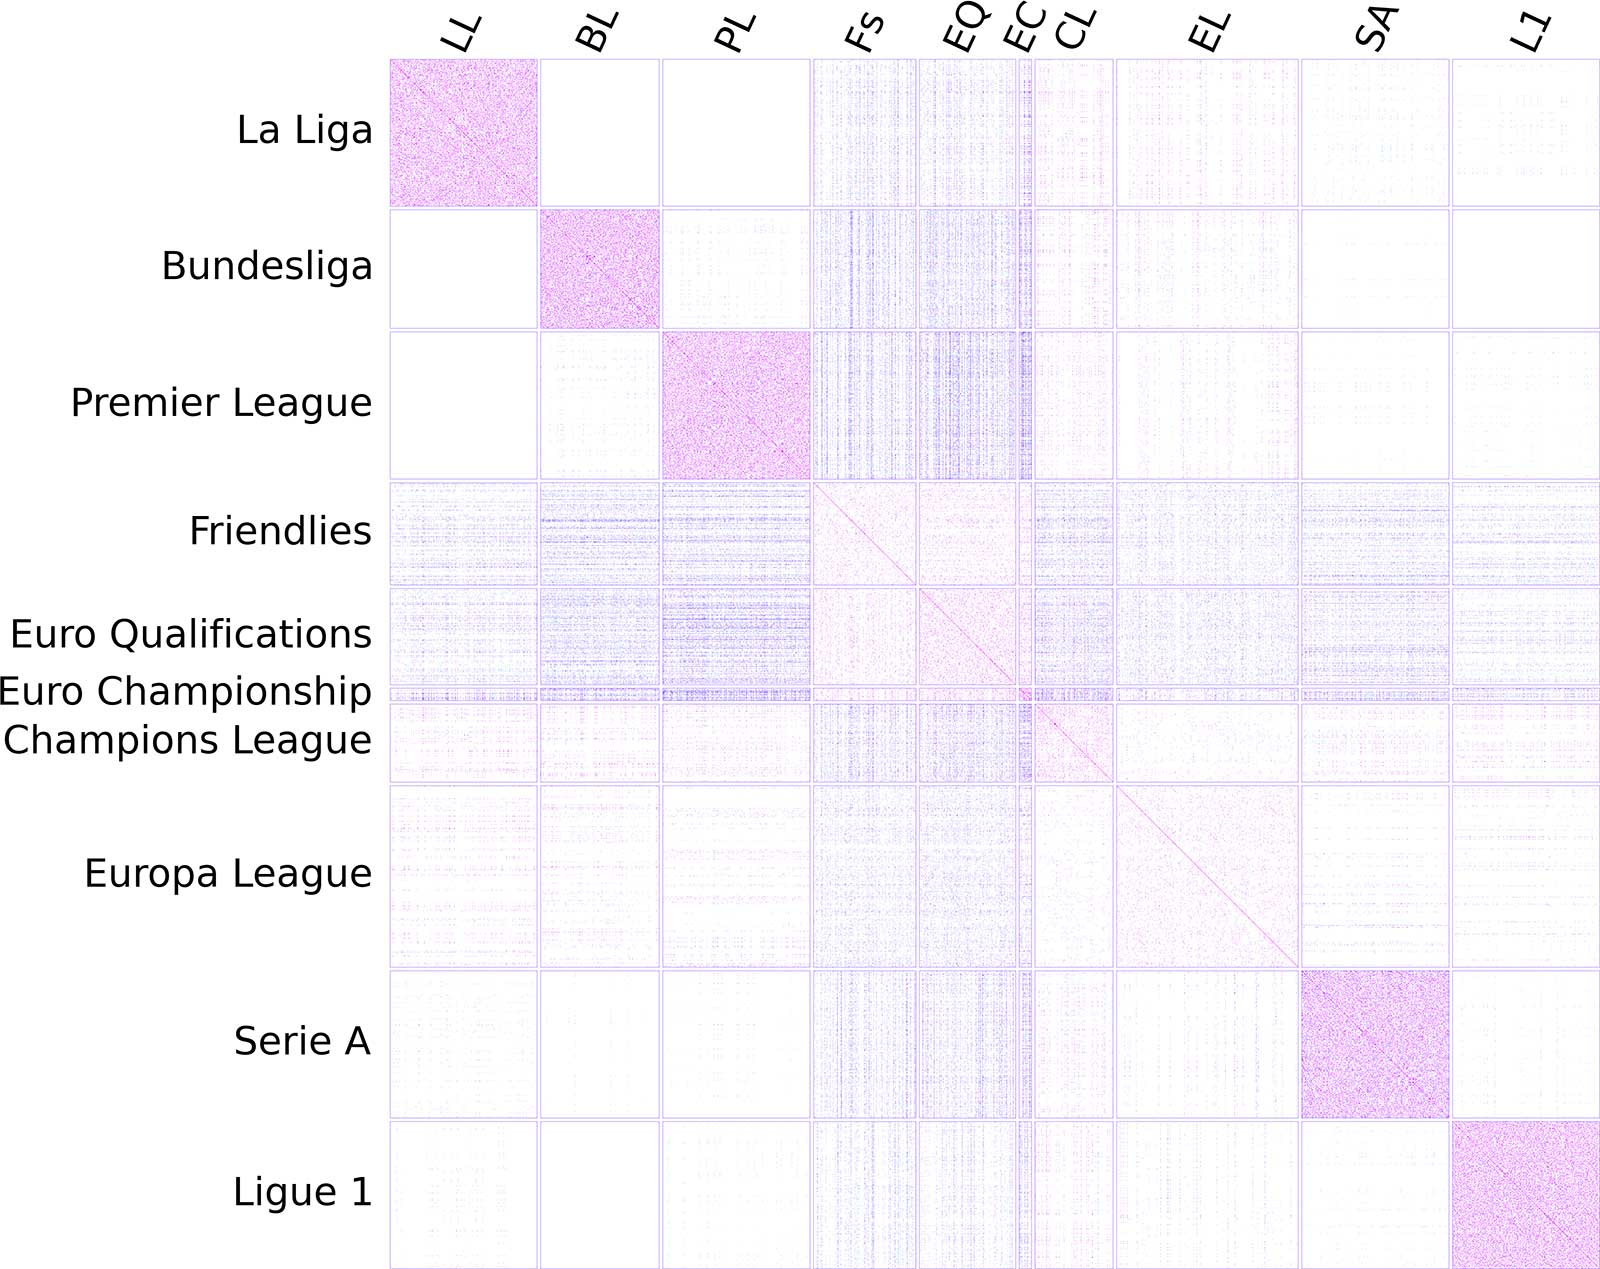
\includegraphics{pk-kernelmatrix}
  \caption{Heatmap of the magnitude of the kernel matrix for \num{3184} matches played over the year preceding Euro 2012.
White indicates zero correlation, a saturated color indicates more correlation.
Matches between national teams exhibit non-zero covariance with matches of all other competitions.
}
  \label{pk:fig:kernel}
\end{figure}

It is interesting to note that the player kernel corresponds to a linear model over the players.
That is, it is equivalent to assuming that there is one independent skill parameter per player, and that the strength of a team is the sum of its players' skills.
Such a model contains a massive number of parameters (possibly much more than the number of observations), and there is little hope to reliably estimate every parameter.
In fact, we observe that the model is ``weakly'' parametric: the number of distinct players usually grows with the number of matches observed.
The kernel-based viewpoint that we take emphasizes the fact that estimating these parameters is not necessary.

\paragraph{Relation to TrueSkill}
Our Gaussian process model coupled to the player kernel is very similar to TrueSkill \citep{herbrich2006trueskill}.
The most important difference is that we take advantage of the dual representation and operate in the space of matches instead of the space of players.
Beyond the conceptual reasons outlined above, it makes inference significantly less computationally intensive for the datasets that we consider.

\section{Experimental Evaluation}
\label{pk:sec:evaluation}

In this section, we evaluate our predictive model on the matches of the Euro 2008, 2012 and 2016 final tournaments and compare it to several baselines.

We collect a dataset of matches from
\begin{enuminline}
\item official and friendly competitions involving national teams, and
\item the most prestigious European club competitions,
\end{enuminline}
starting from July 1\textsuperscript{st}, 2006.
The list of competitions is displayed in Table~\ref{pk:tab:competitions}.
There are approximately $15 \times$ more matches between clubs than there are matches between national teams in our dataset.
With respect to the model outlined in Section~\ref{pk:sec:methods}, our final predictive model processes one additional feature that encodes which team played at home (this feature is null for matches played on neutral ground).
We train the model using a dataset $\mathcal{D}$ consisting of all $M$ matches that were played prior to the start of the competition on which we test.
When computing the kernel matrix (whether on training or on test data) we use the starting lineups, usually announced shortly before the start of the match.
It is interesting to note that the number of distinct players $P$ appearing in the dataset exceeds the number of training instances in each case (the values of $M$ and $P$ are shown in Table~\ref{pk:tab:eval}).

Starting from a Gaussian prior distribution over the $M$ matches $\bm{f} = [f_1 \ \cdots \ f_M]^\Tr \sim \DNorm{\bm{f} \mid \bm{m}, \bm{K}}$, we seek to find the posterior distribution
\begin{align*}
p(\bm{f} \mid \mathcal{D}) \propto \DNorm{\bm{f} \mid \bm{m}, \bm{K}} \prod_{m = 1}^M \frac{1}{1 + \exp(- f_m)}.
\end{align*}
This distribution is intractable, and we use the expectation propagation algorithm\footnote{%
We use the GPy Python library (see: \url{https://sheffieldml.github.io/GPy/}) to fit the model; inference takes a minute for the 2008 test set (17 minutes for 2016).}
to approximate it by a multivariate normal distribution \citep{minka2001family}.
Once the posterior is computed, we can use it to generate predictions for new matches \citep{rasmussen2006gaussian}.
These predictions come in the form of probability distributions $[p^{\text{W}}, p^{\text{D}}, p^{\text{L}}]$ over the three outcomes (win, draw, loss).

\begin{table}
  \caption{
List of competitions included in the dataset, spanning matches from 2006 to 2016.
The majority of matches are played in competitions between clubs.}
  \label{pk:tab:competitions}
  \centering
  \begin{tabular}{llc}
    \toprule
    Competition           & Country       & Involves clubs      \\
    \midrule
    Bundesliga            & Germany       & $\bullet$     \\
    Confederations Cup    & International & \\
    EC Qualification      & International & \\
    European Championship & International & \\
    Friendlies            & International & \\
    Ligue 1               & France        & $\bullet$     \\
    Premier League        & England       & $\bullet$     \\
    La Liga               & Spain         & $\bullet$     \\
    Serie A               & Italy         & $\bullet$     \\
    UEFA Champions League & International & $\bullet$     \\
    UEFA Europa League    & International & $\bullet$     \\
    World Cup             & International & \\
    \bottomrule
  \end{tabular}
\end{table}

We compare our predictive distributions against three baselines.
First, we consider a simple Rao-Kupper model based on national team ratings obtained from a popular Web site\footnote{See: \url{http://www.eloratings.net/}.}.
This model is similar to ours, but
\begin{enuminline}
\item it does not relate matches through players, and thus does not consider club outcomes, and
\item as ratings are fixed values, it does not consider uncertainty in the ratings.
\end{enuminline}
Second, we consider average probabilities derived from the odds given by three large betting companies.
Third, we consider a random baseline which always outputs $[1/3, 1/3, 1/3]$.
The predictive distributions are evaluated using the average logarithmic loss over $T$ test instances
\begin{align*}
- \frac{1}{T} \sum_{i=1}^{T} \left[
\Indic{y_i = \text{W}} \log p^{\text{W}}_i
+ \Indic{y_i = \text{D}} \log p^{\text{D}}_i
+ \Indic{y_i = \text{L}} \log p^{\text{L}}_i
\right].
\end{align*}
The logarithmic loss penalizes more strongly predictions that are both confident and incorrect.
Table~\ref{pk:tab:eval} summarizes the results.




\begin{table}
  \caption{
  Average logarithmic loss of our predictive model (PlayerKern), a model based on national team ratings (Elo), betting odds (Odds) and a random baseline (Random) on the final tournaments of three European championships.
  $M$ is the number of training instances, $P$ the number of distinct players and $T$ the number of test instances.}
  \label{pk:tab:eval}
  \centering
  \begin{tabular}{
    l
    *{2}{S[table-format=5]}
    S[table-format=2]
    *{4}{S[table-format=1.3]}
  }
    \toprule
    Competition &   $M$ &   $P$ & $T$ &    {PlayerKern} &           {Elo} &          {Odds} & {Random} \\
    \midrule
    Euro 2008   &  4390 &  7875 &  31 &           0.969 & \bfseries 0.910 &           0.979 &    1.099 \\
    Euro 2012   & 15594 & 21735 &  31 & \bfseries 0.939 &           1.003 &           0.953 &    1.099 \\
    Euro 2016   & 24887 & 33157 &  51 &           1.067 &           1.102 & \bfseries 1.020 &    1.099 \\
    \bottomrule
  \end{tabular}
\end{table}

Our predictive model performs well in 2008 and 2012, but slightly less so in 2016.
It is noteworthy that the 2016 final tournament has been generally less predictable than earlier editions.
The case of the Elo baseline is interesting, as its accuracy varies wildly.
Reasons for this might include the noise due to the online gradient updates, and the lack of proper uncertainty quantification in the ratings.
Our method, in contrast, seems to produce more conservative predictions, but manages to achieve a more consistent performance.

\section{Summary}
\label{pk:sec:summary}

In this short chapter, we have exposed a connection between a well-known pairwise comparison model and Gaussian-process classification, and have proposed a kernel that is able to transfer knowledge across different types of football matches---those between clubs and those between national teams.
We have shown that a predictive model built on these ideas achieves a logarithmic loss that is competitive with betting odds.
In future work, we would like to investigate how to incorporate aging into the model, i.e., how to progressively downweight older data.

